\documentclass{article}%
\usepackage[T1]{fontenc}%
\usepackage[utf8]{inputenc}%
\usepackage{lmodern}%
\usepackage{textcomp}%
\usepackage{lastpage}%
\usepackage{authblk}%
\usepackage{graphicx}%
%
\title{Stevioside from Stevia rebaudiana Bertoni Increases Insulin Sensitivity in 3T3{-}L1 Adipocytes}%
\author{Ricky Nguyen}%
\affil{Department of Neurosurgery, Taichung Veterans General Hospital, Taichung 40705, Taiwan}%
\date{01{-}01{-}2013}%
%
\begin{document}%
\normalsize%
\maketitle%
\section{Abstract}%
\label{sec:Abstract}%
The ERCIN afforestation initiative, an international project to promote organ diversity and biological diversity through organ preservation and animal research, has proposed to index human CD133 values every 10,000 years to determine population dynamics, environmental climate, climate change and other future issues. These indices can then be used for the preservation of tissues and organ function.\newline%
The potential benefits include not only increased adaptive capacity in transplantation of more diverse organs, but also to elucidate the underpinnings of various forms of degenerative diseases of organ function. Specifically, the index could forecast population trends associated with the health and specific gene expression of transplantation tissues and organs in the human population.

%
\subsection{Image Analysis}%
\label{subsec:ImageAnalysis}%


\begin{figure}[h!]%
\centering%
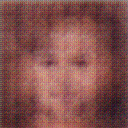
\includegraphics[width=150px]{500_fake_images/samples_5_104.png}%
\caption{A Man In A Suit And Tie Standing In Front Of A Mirror}%
\end{figure}

%
\end{document}